\chapter{Parkinson}
\section{Definição}

A Doença de Parkinson (DP) é caracterizada por ser uma doença crônica, progressiva e degenerativa do sistema nevorso central, reconhecida principalmente por distubios motores \cite{souzametodos}, como a bradicinesia, tremores corpoais em repouso e rigidez corporal \cite{da2016aspectos}, A bradicinesia é a redução da movimentação ou seja o indivíduo consegue se movimentar porém lentamente. A DP é resultante da degeneração lenta e severa dos neurônios dopaminérgicos da substância negra ~\ref{substanciaNegra}, responsável pela produção de dopamina um neurotransmissor fundamental para a gestão dos movimentos \cite{eftaxias2015detection}.

\begin{figure}[!htb]
   \centering
    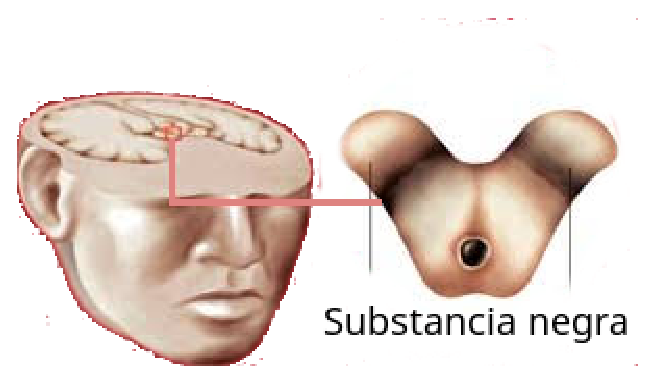
\includegraphics[width=0.8\textwidth]{figuras/substancia_negra.eps}
    \caption{Esquematização da substância negra.}
    \label{substanciaNegra}
\end{figure}

\section{Diagnóstico e Sintomas}
A doença de Parkinson afeta aproximadamente entre 1\% a 2\% da população mundial acima dos 65 anos, sendo que no Brasil atinge entorno de 3\% da população nesta faiza etaria. \cite{magalhaes2009descobrindo}, tendo a idade como o único fator de risco conhecido, a DP é rara antes dos 40 anos, aumenta após os 50 e é tem maior probabilidade após os 70 anos \cite{peixinho2006alteraccoes}, porém a incidência da doença não está restrita somente a pessoas idosas, uma vez que 20\% dos casos são de pessoas com menos de 50 anos \cite{gago2014manual}, não há consenso estabelecido, mas alguns estudos relacionam ser um pouco maior a ocorrência no sexo masculino \cite{peixinho2006alteraccoes}.

O diagnóstico da DP atualmente é clínico realizado pelo Neurologista, onde identifica-se:
\begin{itemize}
    \item bradicinésia (lentidão dos movimentos).
    \item Tremor em repouso.
    \item Rigidez muscular.
    \item Instabilidade postural.
\end{itemize}

Para realizar o diagnóstico identifica-se a bradicinésia e pelo menos um de três outros sintomas, tremor em repouso, rigidez muscular ou instabilidade postural \cite{gago2014manual}. Também pode ser utilizado para confirmar a DP exames como Tomografia computadorizada e ressonância magnética cerebral dentre outros a ser prescrito pelo Neurologista \cite{gago2014manual}.

Outros sintomas recorrentes são associados a comunicação oral, onde 90\% dos pacientes possuem problemas relacionados a fala, como gagueira, rouquidão, alteração ou enfraquecimento da voz \cite{zarzur2010laryngeal}, outro sintoma relevante é a demência que cerca de 25\% dos pacientes \cite{pamplona1996demencia}\%, também podem ocorrer alterações do sono de memória e depressão\cite{barbosa2005parkinsons}.

\subsection{Tratamento}
A Doença de Parkinson não tem cura, consequentemente os tratamentos disponíveis visam a melhora da qualidade de vida do paciente controlando os sintomas, com o objetivo de aumentar ao máximo autonomia e independência do paciente relacionada a doença. Existem vários tipos de tratamentos sendo essencial uma equipe multiprofissional, para atendimentos específicos para cada tipo de sintoma apresentado \cite{saito2011doencca}.

